\chapter{Konstrukcja robota}

Do konstrukcji robota została zakupiona platforma \textit{4WD Outdoor Mobile Platform}. Składa się ona metalowej obudowy oraz czterech silników i kół \cite{Outdoor_robot}. Posiada ona poziomowy charakter budowy, jednakże konstruowany robot składa się tylko z dolnego poziomu. 

Głównym założeniem mechanicznym jest stworzenie jeżdżącego robota mobilnego poruszającego się po środowisku lądowym. Ruch robota jest możliwy zarówno po płaskiej i nierównej powierzchni. Podzespoły robota można podzielić na  układ napędowy, układ sterujący, czujniki oraz zasilanie.



\section{Komunikacja podzespołów}

Sposób komunikacji podzespołów został przedstawiony na Rys. \ref{fig:schemat}. 

Jednostka mocy Pololu Dual VNH5019 jest dwukanałowa. Oznacza to, że możliwe jest sterowanie prędkością po dwóch stronach robota, a nie na każdym kole. Silniki po tej samej stronie zostały połączone szeregowo, a następnie trwale połączone z  jednostką mocy, która z kolei została połączona z mikro kontrolerem. 

Napięcie znamionowe dla STM32L476RG  wynosi od 1.71 do 3.6V, natomiast napięcie sygnałów A i B pochodzących od enkoderów przyjmuje wartość 5V. W tym celu został wykorzystany konwerter poziomów, który zmniejszył ich napięcie do 3.3V, które jest bezpieczne dla użytego mikro kontrolera.

Z mikro kontrolerem łączy się dodatkowo, poprzez komunikacje I2C, jednostka inercyjna MPU9250. STM32 komunikuje się poprzez port szeregowy z głównym sterownikiem. Up Board otrzymuje ponadto dane z dedykowanego systemu wizyjnego, połączonego poprzez USB 3.0 OTG i lidaru połączonego poprzez USB 2.0. Dodatkowo na zewnątrz urządzenia został wyprowadzony Qilive Hub z 4 portami USB 2.0. Pozwali to na rozbudowanie robota o kolejne moduły bez konieczności ingerencji elektronikę znajdującą się wewnątrz obudowy.

Główny sterownik wymienia informacje ze zdalnym komputerem poprzez wi-fi. Wykorzystany do tego został zdalny moduł wi-fi ASUS WL-167g, jest on połączony z główny sterownikiem poprzez USB 2.0.

\begin{figure}[!ht]
	\centering
	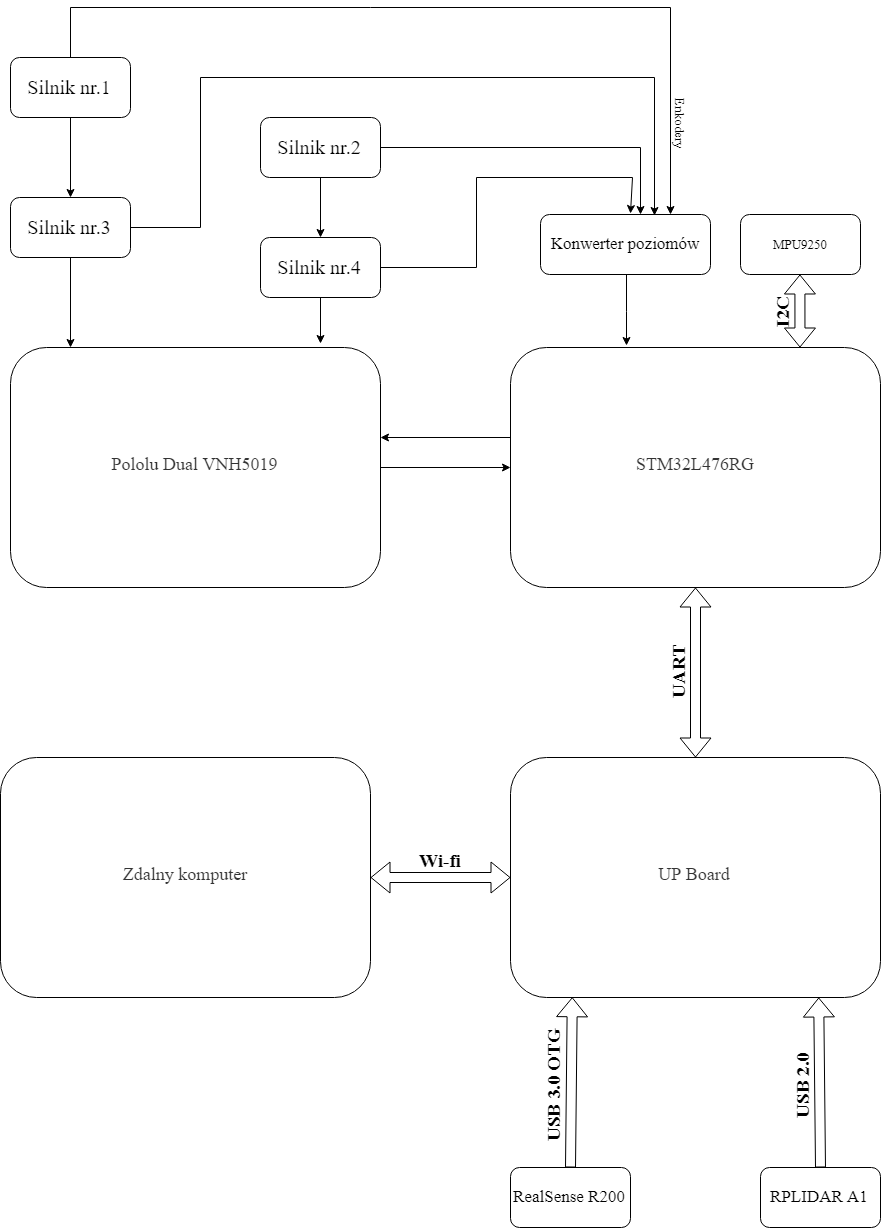
\includegraphics[scale=0.5]{schemat.png}
	\caption{Schemat komunikacji podzespołów.}
	\label{fig:schemat}
\end{figure}


\section{Układ napędowy}
Elementami wykonawczymi robota są części napędowe, czyli silniki DC. Nadają one kołom prędkość obrotową zadaną sterowaniem otrzymanym z układu sterującego. Wykorzystane silniki są dedykowanymi elementami do wykorzystanej obudowy robota.
\subsection{Silniki prądu stałego}

Napęd robota stanowią 4 silniki prądu stałego zintegrowane z przekładnią zębatą  i połączone z enkoderami kwadratowymi (Rys.\ref{fig:silnik}). Oznaczenie modelu to No.GB37Y3530-12V-251R. Przełożenie przekładni wynosi 43,8:1. Enkoder kwadratowy zapewnia rozdzielczość 16 pomiarów na obrót wału silnika co odpowiada 700 pomiarom na obrót wału wyjściowego. Oznacza to, że impuls będzie występował co 0.6mm przebytej drogi. Najważniejsze dane techniczne silnika zostały przedstawione w tabeli \ref{parametry_silnika}.


\begin{figure}[ht]
	\centering
	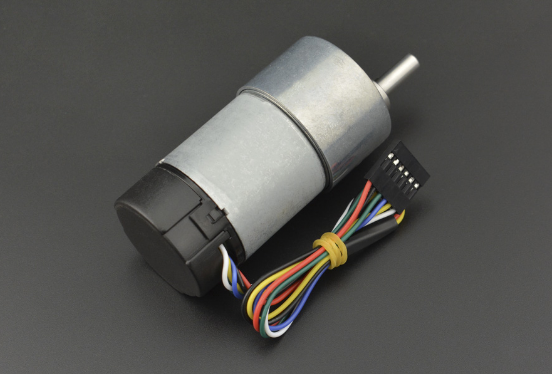
\includegraphics[scale=0.7]{silnik.png}
	\caption{Silnik DC serii Gear Motor.}
	\label{fig:silnik}
\end{figure}



\begin{table}[]
	\centering
	\caption{Parametry silnika.}
	\label{parametry_silnika}
	\begin{tabular}{|c|c|}
		\hline
		\multicolumn{2}{|c|}{\textbf{Specyfikacja}} \\ \hline
		Napięcie zasilania                & 1 - 12V \\ \hline
		Natężenie prądu bez obciążenia    & 350mA   \\ \hline
		Prędkość obrotowa bez obciążenia  & 251RPM  \\ \hline
		Napięcie znamionowe enkodera      & 5V      \\ \hline
		Typ enkodera                      & Hall    \\ \hline
		Waga                              & 205g    \\ \hline
	\end{tabular}
\end{table}

\subsection{Koła}

Do poruszania się robota zostały wykorzystane koła o średnicy \i134mm i szerokości 48mm z gumową oponą terenową(Rys. \ref{fig:koła}). Szeroka opona zapewnia  większą powierzchnię styku z podłożem. Skutkuje to uzyskaniem lepszej przyczepności oraz skróceniem drogi hamowania w stosunku do węższej opony.
\begin{figure}[ht]
	\centering
	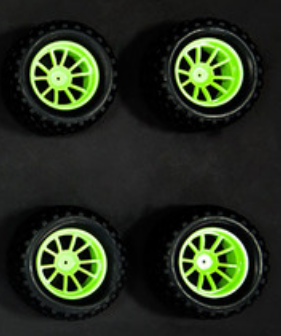
\includegraphics[scale=0.8]{koła.png}
	\caption{Koła robota.}
	\label{fig:koła}
\end{figure}

Dobrane silniki i koła pozwalają robotowi mobilnemu na uzyskanie maksymalnej prędkości równej ok. 1.5$\frac{m}{s}$. Osiągana prędkość jest wystarczająca do planowanych zastosowań robot.

\section{Układ sterujący}

Układ sterujący ma na celu wyznaczenie i zadanie sterowania na elementy wykonawcze. W tym przypadku będzie to zadawanie  prędkości obrotowej na koła, poprzez zmianę wartości natężenia prądu podawanego na silniki.  Wykorzystany w tym celu został dwukanałowy układ mocy, mikro kontroler oraz nadrzędny sterownik główny. Na zdalnym komputerze jest wyliczana prędkości liniowa i kątowa, którą ma osiągnąć robot. Informację tę pobiera mikro kontroler i na jej podstawie przelicza prędkość z jaką mają się poruszać prawe i lewe koła. Następnie przy pomocy układu mocy prąd o odpowiednim natężeniu jest podawany na silniki. 


\subsection{Układ mocy}

Do sterowania napędami zastosowany został układ mocy Pololu Dual VNH5019 Motor Driver Shield (Rys.\ref{fig:pololu}). Układ ten jest kompatybilny z platformą Arduino. Posiada własną bibliotekę, która pozwala w bardzo prostu sposób sterować silnikami prądu stałego zasilane napięciem z zakresu 5.5 - 24V o ciągłym poborze prądu do 12A.  Posiada dwa kanały do sterowania silnikami, do każdego kanału zostały wpięte dwa silniki znajdujące się po tej samej stronie, połączone w sposób równoległy.   

Układ umożliwia zmianę kierunku obrotów silnika oraz regulacje prędkości obrotowej poprzez sygnał PWM. Działanie poszczególnych pinów zostało przedstawione w Tabeli \ref{pololu_pins}.

\begin{figure}[ht]
	\centering
	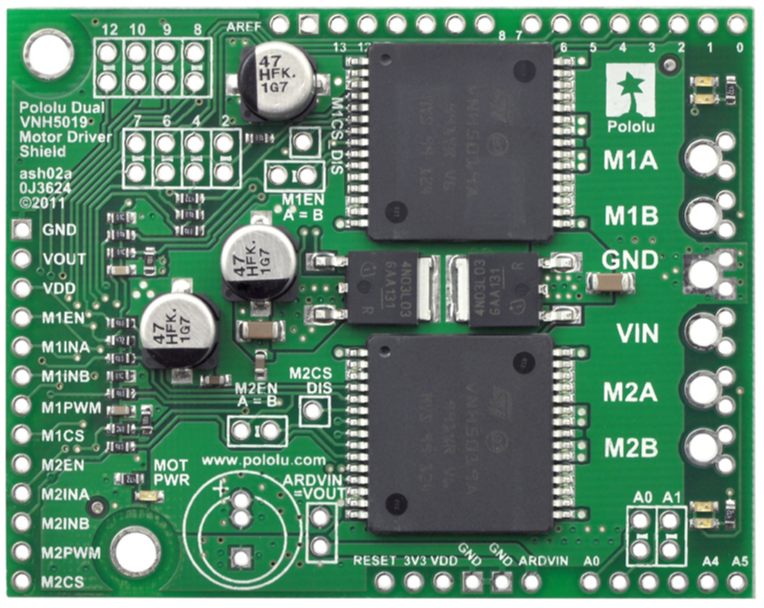
\includegraphics[scale=0.6]{pololu.png}
	\caption{Pololu Dual VNH5019 Motor Driver Shield.}
	\label{fig:pololu}
\end{figure}



\begin{table}[!h]
	\centering
	\caption{Piny sterownika silników.}
	\label{pololu_pins}
	\begin{tabular}{|c|c|}
		\hline
		\textbf{VNH5019 Pin} & \textbf{Zastosowanie}           \\ \hline
		M1INA                & Kierunek silnika 1 - wejście A  \\ \hline
		M1INB                & Kierunek silnika 1 - wejście B  \\ \hline
		M1EN/DIAG            & Silnik 1 – informacja o błędzie \\ \hline
		M2INA                & Kierunek silnika 2 – wejście A  \\ \hline
		M2INB                & Kierunek silnika 2 – wejście B  \\ \hline
		M1PWM                & Sterowanie prędkością silnika 1 \\ \hline
		M2PWM                & Sterowanie prędkością silnika 2 \\ \hline
		M2EN/DIAG            & Silnik 2 – informacja o błędzie \\ \hline
		M1CS                 & Odczyt prądu na silniku 1       \\ \hline
		M2CS                 & Odczyt prądu na silniku 2       \\ \hline
	\end{tabular}
\end{table}




\subsection{Mikrokontroler}


Do sterowania robotem wykorzystany został mikro kontroler  STM32 Nucleo-L476RG(Rys.\ref{fig:stm32}) z wydajnym rdzeniem Arm® Cortex®-M4 32-bit RISC, taktującym do 80Mhz. Wyposażony jest w 1MB pamięci flash oraz 128KB pamięci SRAM. Obsługuje interfejsy komunikacyjne takie jak SPI, I2C, USART, UART, USB, CAN. Posiada wbudowany programator i debugger ST-LINK/V2-1. Pozwala na prace w trybie kompatybilności z Arduino Uno, pozwala to wykorzystywać do jego programowania środowiska dedykowane językowi Arduino. Umożliwia obsługę szesnastu liczników różnorakiego zastosowania. Posiada 51pinów typu GPIO(\textit{general-purpose input/output}), a także 16 linii przerwań zewnętrznych. Źródłem zasilania jest przez port USB z napięciem między 3.0-3.6V.

\begin{figure}[ht]
	\centering
	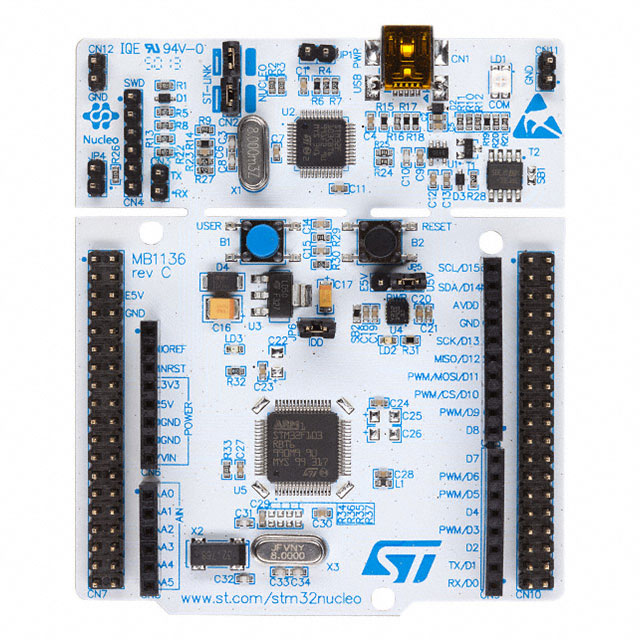
\includegraphics[scale=0.40]{stm32.png}
	\caption{Mikrokontroler STM32 Nucleo-L476RG.}
	\label{fig:stm32}
\end{figure}

Zastosowany mikro kontroler pozwolił na integrację z jednostką mocy, ponieważ jego budowa umożliwia pracę w trybie kompatybilnym z Arduino Uno. Wykorzystany STM pozwala więc na wykorzystanie bibliotek dostępnych dla Arduino, ale dodatkowo oferuje większą pamięć podręczną i moc obliczeniową. Znaczącą zaletą jest także duża liczba pinów GPIO. Zostały one wykorzystane do uzyskania komunikacji z enkoderami, jednostką inercyjną, a także jednostką mocy. 

W dokumentacji technicznej mikro kontrolera zostały odnalezione piny odpowiedzialne za poszczególne funkcje, a następnie stworzono schemat wszystkich potrzebnych połączeń(Tabela. \ref{stm_pins}). Połączenia związane z enkoderami i jednostką inercyjną zostały trwale wykonane na płytce prototypowej do lutowania, natomiast piny związane z jednostką mocy posiadają możliwość wyjęcia.  

% Please add the following required packages to your document preamble:
% \usepackage{graphicx}
\begin{table}[ht]
	\centering
	\caption{Połączenia pinów STM32 Nucleo-L476RG. }
	\label{stm_pins}
	\begin{tabular}{|c|c|}
		\hline
		\textbf{STM32 Pin} & \textbf{Zastosowanie} \\ \hline
		PA10               & VNH5019  - M1INA      \\ \hline
		PB5                & VNH5019 - M1INB       \\ \hline
		PB10               & VNH5019 - M1EN/DIAG   \\ \hline
		PA8                & VNH5019 - M2INA       \\ \hline
		PA9                & VNH5019 - M2INB       \\ \hline
		PC7                & VNH5019 - M1PWM       \\ \hline
		PB6                & VNH5019 - M2PWM       \\ \hline
		PA6                & VNH5019 - M2EN/DIAG   \\ \hline
		PA0                & VNH5019 - M1CS        \\ \hline
		PA1                & VNH5019 - M2CS        \\ \hline
		PB13               & MPU9250 - SCL         \\ \hline
		PB14               & MPU9250 - SDA         \\ \hline
		PC8                & Enkoder 1 - Sygnał A  \\ \hline
		PC6                & Enkoder 1 - Sygnał B  \\ \hline
		PC5                & Enkoder 2 - Sygnał A  \\ \hline
		PA12               & Enkoder 2 - Sygnał B  \\ \hline
		PB2                & Enkoder 3 - Sygnał A  \\ \hline
		PB1                & Enkoder 3 - Sygnał B  \\ \hline
		PB15               & Enkoder 4 - Sygnał A  \\ \hline
		PC4                & Enkoder 4 - Sygnał B  \\ \hline
	\end{tabular}
\end{table}

\subsection{Sterownik główny i zdalny komputer}

Jednostką nadrzędną, którą wykorzystuje robot jest minikomputer UP Board(Rys.\ref{fig:upboard}). Główne parametry platformy zostały przedstawione w Tabeli \ref{up_board_specyfikacja}. Wykorzystywany system operacyjny Ubuntu 16.04.6 LTS. System ten jest kompatybilny z pakietem ROS Kinetic Kame, w oparciu o niego odbywa się komunikacja między wszystkimi modułami. Zdalny komputer także posiada zainstalowany ten sam system oraz tę samą wersje pakietu ROS, pozwoli to na wykorzystanie komunikacji między wątkowej. 

\begin{figure}[ht]
	\centering
	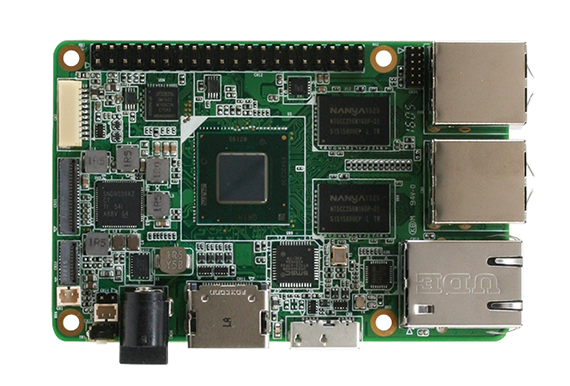
\includegraphics[scale=0.6]{upboard.png}
	\caption{Minikomputer Up Board}
	\label{fig:upboard}
\end{figure}

Platforma posiada jeden port USB 3.0 OGT, przez który jest połączona ze swoim dedykowanym systemem wizyjnym. Liczba dostępnych portów USB 2.0 została zwiększona do siedmiu, poprzez wykorzystanie Qilive Hub. Przy ich pomocy odbywa się komunikacja z lidarem, a także mikro kontrolerem. Moduł wi-fi został wyprowadzony na zewnątrz robota, aby zwiększyć siłę sygnału, ponieważ od niej zależy szybkość przesyłu danych do zdalnego komputera. 

Na platformie został zainstalowany także program RealVNC w trybie serwera. Pozwala on na zdalny dostęp do minikomputera przez wi-fi ze zdalnego komputera, na którym jest zainstalowany pakiet RealVNC w trybie obserwatora. RealVNC na minikomputerze jest uruchamiany przy starcie systemu, dzięki temu zdalny komputer posiada dostęp do \textit{pulpitu} od momentu uruchomienia całego robota. Prędkość transmisji zdalnego obrazu zależy od prędkości sieci na komputerze pokładowym, sprawia to problemy przy słabej jakości połączenia. 

Zasilanie odbywa się z wykorzystaniem przetwornicy napięcia, podłączonej na stałe do wyprowadzeń na płytce. Pozwoliło to na zasilanie platformy z tego samego źródła co napędy. Up Board nie posiada przełącznika odpowiadającego za uruchamianie. Sprawia to, że w momencie podłączenia zasilania uruchamia się samoistnie.
\begin{table}[h]
	\centering
	\caption{Specyfikacja minikomputera Up Board.}
	\label{up_board_specyfikacja}
	\resizebox{\textwidth}{!}{%
		\begin{tabular}{|c|c|}
			\hline
			\multicolumn{2}{|c|}{\textbf{Specyfikacja}}                                                                                                         \\ \hline
			Procesor   & Intel® Atom™ x5-Z8350 Processor (2M Cache, do 1.92 GHz) 64-bitowy,4-rdzeniowy                                                          \\ \hline
			Pamięć RAM & 1GB / 2GB / 4GB DDR3L-1600                                                                                                             \\ \hline
			Dysk eMMC  & 16GB / 32 GB / 64 GB                                                                                                                   \\ \hline
			Grafika    & Intel® HD 400 Graphics                                                                                                                 \\ \hline
			Złącza     & \begin{tabular}[c]{@{}c@{}}4x gniazdo USB 2.0 \\ 2x wyprowadzenie USB 2.0\\ 1x gniazdo USB 3.0 OTG\\ 1x gniazdo HDMI 1.4a\end{tabular} \\ \hline
			Wymiary    & 85.60mm x 56.5mm                                                                                                                       \\ \hline
			Zasilanie  & 5V DC-in                                                                                                                               \\ \hline
		\end{tabular}%
	}
\end{table}

\section{Układ pomiarowy}

Układ pomiarowy służy do mierzenia wybranych wartości fizycznych. Pozwala on na uzyskanie informacji o zachowaniu systemu pod wpływem zadanego sterowania. W budowie robota zostały wykorzystane: system wizyjny, jednostka inercyjna oraz lidar. Wysyłają one informacje na temat otoczenia, a także prędkości i przyśpieszenia robota.
\subsection{System wizyjny}

Wykorzystanym systemem wizyjnym jest dedykowana dla Up Board kamera Intel RealSense R200(Rys. \ref{fig:realsense}).  Najważniejsze dane techniczne zostały przedstawione w Tabeli \ref{kamera}.Dzięki interfejsowi USB 3.0 OTG prędkość przesyłu danych jest wystarczająca na uzyskanie obrazu otoczenia w czasie rzeczywistym. Posiada także bibliotekę umożliwiającą jej komunikację między wątkową ROS.

\begin{figure}[ht]
	\centering
	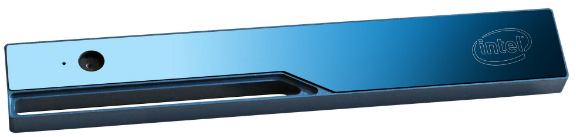
\includegraphics[scale=0.6]{realsense.png}
	\caption{RealSense R200.}
	\label{fig:realsense}
\end{figure}

\begin{table}[]
	\centering
	\caption{Parametry kamery.}
	\label{kamera}
	\begin{tabular}{|c|c|}
		\hline
		\multicolumn{2}{|c|}{\textbf{Specyfikacja}}               \\ \hline
		Zakres pracy                    & 0.5m - 3.5m             \\ \hline
		Rozdzielczość głębokości        & 480 x 360               \\ \hline
		Szybkość w kl/s                 & 60fps                   \\ \hline
		Głębia ostrości i pola widzenia & H: 59, V: 46, D: 70     \\ \hline
		Typ interfejsu systemu          & USB 3.0                 \\ \hline
		Wymiary                         & 101.6mm x 9.6mm x 3.8mm \\ \hline
	\end{tabular}
\end{table}


\subsection{Jednostka inercyjna}

Wykorzystana jednostka inercyjna to MPU-9250(Rys. \ref{fig:imu}), jest to urządzenie 9-osiowe, które wyposażone jest w 3-osiowy żyroskop, 3-osiowy akcelerometr i 3-osiowy magnetometr. Posiada także czujnik temperatury.  Umożliwia komunikację magistralami I2C oraz SPI. W przypadku rozważanego robota wykorzystany został interfejs I2C. Żyroskop informuje o prędkości kątowej robota, pozwala on na ustalenie orientacji. Akcelerometr podaje informacje na temat wypadkowej siły działającej na platformę. W przypadku braku zewnętrznych sił robot jest poddany działaniu tylko siły grawitacji, akcelerometr pozwala się na określenie pozycji platformy względem podłoża. Magnetometr dostarcza informacji na temat ziemskiego pola magnetycznego. MPU-9250 posiada własną bibliotekę Arduino ułatwiającą odczyt danych z czujników.

\begin{figure}[h]
	\centering
	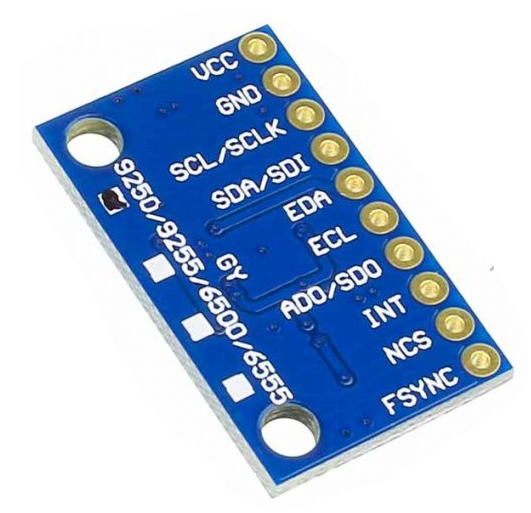
\includegraphics[scale=0.4]{imu.png}
	\caption{Jednostka inercyjna MPU-9250.}
	\label{fig:imu}
\end{figure}

\subsection{Lidar}

Lidar(\textit{Light Detection and Ranging}) jest skanerem laserowym, który pozwala na detekcję elementów otoczenia i poznania odległości od nich. Umożliwia to wykonanie mapy środowiska które jest skanowane przez lidar.

W robocie mobilnym został zamontowany RPLIDAR A1(Rys. \ref{fig:lidar}), jest to  lidar, z możliwością obrotu o 360 stopni. Posiada zasięg do 12m i częstotliwości do 10Hz. Komunikacja następuje przez interfejs UART, połączony z jednostką nadrzędną przez port USB 2.0. Wyposażony jest w dedykowaną bibliotekę do komunikacji między wątkowej ROS.

\begin{figure}[h]
	\centering
	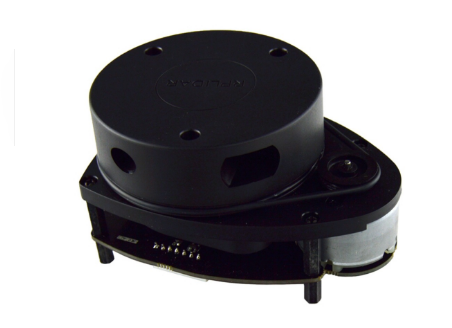
\includegraphics[scale=0.7]{lidar.png}
	\caption{Skaner laserowy RPLIDAR A1.}
	\label{fig:lidar}
\end{figure}



\section{Zasilanie}


Zasilanie konieczne jest dla silników napędowych i platformy Up Board. W tym celu został wykorzystany akumulator litowo-polimerowy Gens Ace 3700mAh 14.8V z serii TATTU(Rys. \ref{fig:lidar}). Jego prąd rozładowania wynosi 45C. Umieszczony jest na zewnątrz robota w celu wygodnego dostępu do ładowania. Połączony jest z układem mocy VNH5019 oraz przetwornicą napięcia w celu obniżenia do 5V, aby możliwe było zasilenie minikomputera Up Board.

\begin{figure}[h]
	\centering
	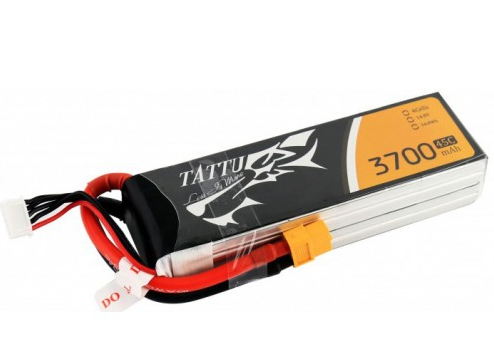
\includegraphics[scale=0.7]{bateria.png}
	\caption{Akumulator z serii TATTU.}
	\label{fig:bateria}
\end{figure}

